\documentclass{article}

\usepackage[preprint]{neurips_2023}

\usepackage[T1]{fontenc}
\usepackage[utf8]{inputenc}
\usepackage{microtype}
\usepackage{amsmath,amssymb,mathtools}
\usepackage{graphicx}
\graphicspath{{./}{../}}
\usepackage{booktabs}
\usepackage{float}
\usepackage{enumitem}
\usepackage{hyperref}
\usepackage{cleveref}

\newcommand{\fomc}{FOMC}
\newcommand{\fed}{Federal Reserve}
\newcommand{\tfidf}{TF--IDF}
\newcommand{\svm}{linear SVM}
\newcommand{\logreg}{logistic regression}
\newcommand{\code}[1]{\texttt{#1}}

\newcommand{\reportfigure}[3]{
\begin{figure}[H]
    \centering
    \includegraphics[width=#2\textwidth]{#1}
    \caption{#3}
\end{figure}
}

\title{
Inflation versus Labor-Market Attention in FOMC Statements and Minutes\\
\large A descriptive NLP report on the Federal Reserve dual mandate, 2000--2024
}

\author{
  Kamil Stos \\
  ENSAE Paris \\
  \texttt{kamil.stos@ensae.fr}
}

\begin{document}

\maketitle

\begin{abstract}
This report studies how \fomc{} statements and minutes differ in their treatment of the
two sides of the Federal Reserve's mandate: inflation and the labor market. The corpus
contains 199 meetings from 2000 to 2024, with one statement and one set of minutes for
each meeting. I start from a transparent dictionary score: inflation language minus
labor-market language, normalized by document length. In this sample, statements are
shorter, more concentrated, and more inflation-dominant than minutes. Minutes are longer
and closer to balance, with more space for labor-market conditions, uncertainty, and
financial stress. I then move to sentences. A balanced sample of sentences is labelled
with a local language model and used as a weakly annotated training set. Simple sentence
classifiers based on \tfidf{} and local embeddings are trained to distinguish inflation,
labor, financial-conditions, policy-decision, and other sentences. The embedding
classifier agrees more closely with the weak labels than the dictionary rule and gives a
useful second view of the corpus. The results should be read descriptively: the
dictionary remains the main interpretable measure, while the sentence model shows where
exact keyword matching misses broader financial-conditions language.
\end{abstract}

\section*{Introduction}
\label{sec:introduction}

The \fed{} has a dual mandate: price stability and maximum employment. After each
\fomc{} meeting, the Committee publishes a short statement. A few weeks later, it
publishes longer minutes. Both documents refer to the same meeting, but they play
different communication roles. The statement is the immediate public message; the minutes
give a more detailed account of the discussion.

This report asks a simple question:

\begin{quote}
\emph{Do statements and minutes give the same relative attention to inflation and the labor market? Do they treat both subjects the same way?}
\end{quote}

We look at the topics that appear in the
documents, the space given to each side of the mandate, and the way this changes across
document types and periods. 

The difference is interesting because the Fed's legal mandate is
dual, but price stability has a privileged place as the initial original mandate. Inflation is
directly tied to credibility, expectations, and the policy instruments. 

This report takes the macro-topic angle: inflation versus the
labor market. The companion report by Mathieu takes the symmetric policy-tone angle: hawkish versus dovish communication.  The two views complement each other. Inflation language often supports a hawkish signal, but the mapping is not exact. Labor-market language can describe 
wage pressure, demand, or resilience while the overall policy stance remains restrictive.

The analysis proceeds in three steps. First, I compare statements and minutes with the
dictionary score across document types, time, policy episodes, and rate decisions. This
gives the main observation that statements are more inflation-heavy than minutes.
Second, I move to sentences and try to understand closer what the dictionary is actually counting. Third,
I use LLM-assisted weak labels to train simple sentence classifiers with \tfidf{} and
embedding features. This last step is more of a
check on whether broader topic categories, especially financial conditions, can be
recovered from sentence text. These different methods are rather used as a sequence of
checks on the same object, to try to catch quirks or different points of view.

\section*{Related Work}
\label{sec:literature}

There is an extensive body of litterature on FOMC communication and especially in relation to financial markets, fixed income instruments and especially Overnight Indexed Swap (OIS) rates  since they are directly translating the market's expectation of the FED's decision.  Tadle
\citep{tadle2022minutes} builds sentiment indices for statements and minutes and relates minutes sentiment to financial-market reactions. 
However, in this report, we focus solely on the language to stay in the scope of the project.


There is still a large body of literature that aims at using text methods to study \fomc{} communication directly. Acosta and
Meade \citep{acosta2015hanging} study post-meeting statements with semantic similarity
methods and document how statements evolved over time. Hansen, McMahon, and Prat
\citep{hansen2018transparency} use computational linguistics on internal \fomc{}
transcripts to study deliberation and transparency inside the Committee. Their data are
richer than mine because transcripts contain individual interventions. This report uses
only public statements and minutes, so it measures the communication that is released to
the public, not the full internal discussion.

The closest paper for the dual-mandate motivation is Shapiro and Wilson
\citep{shapiro2022taking}. They estimate central-bank objectives from the language of
internal meetings, including the relative weight placed on inflation and real activity.
The goal of my report is rather to be descriptive and to get a feel for how both subjects are treated linguistically, not evaluate their economical relevance. 

Doh, Kim, and Yang
\citep{doh2021matters} show that qualitative descriptions in \fomc{} statements can
matter for bond prices. Doh, Song, and Yang \citep{doh2025deciphering} use alternative
\fomc{} statements and language models to measure hawkish and dovish policy stance.
Those papers are closer to the companion report on hawkish versus dovish communication. 


\section*{Data}
\label{sec:data}

The corpus comes from the official \fed{} website and is retrieved and parsed automatically. Each row corresponds to one meeting and contains
the meeting date, URLs, statement text, and minutes text.

The sample contains 199 meetings from February 2000 to December 2024. Every meeting has
both a statement and minutes. Rate decisions are inferred from statement text with simple
regular expressions and coded as \emph{hike}, \emph{cut}, or \emph{hold}. The sample has
59 hikes, 30 cuts, and 110 holds.

\begin{table}[H]
\centering
\caption{Corpus size and document length.}
\label{tab:descriptive}
\begin{tabular}{lrrrr}
\toprule
Document type & Documents & Mean words & Median words & Std. words \\
\midrule
Statements & 199 & 526.1 & 536.0 & 217.4 \\
Minutes    & 199 & 7283.2 & 7536.0 & 2441.3 \\
\bottomrule
\end{tabular}
\end{table}

\reportfigure{figures/document_length_by_type.png}{0.82}
{Document length by meeting. Minutes are much longer than statements, so dictionary scores are normalized by document length.}

Minutes contain about fourteen times more words than
statements on average, so the main
quantities below are reported as mentions per 1,000 words.

We almost don't preprocess the text, it is just lowercased, whitespace is normalized, and then words are counted with a regular expression. Stopwords are kept for the dictionary
measure because several terms are multi-word expressions, such as \emph{price
stability}, \emph{labor market}, and \emph{inflation expectations}.

\subsection*{Dictionary balance}

I define two short dictionaries. The inflation dictionary contains terms such as
\emph{inflation}, \emph{inflationary}, \emph{price stability}, \emph{price pressures},
\emph{inflation expectations}, \emph{core inflation}, \emph{PCE inflation},
\emph{consumer prices}, \emph{energy prices}, \emph{food prices}, \emph{cost pressures},
\emph{supply constraints}, and \emph{disinflation}.

The labor-market dictionary contains terms such as \emph{employment},
\emph{unemployment}, \emph{labor market}, \emph{job gains}, \emph{payrolls},
\emph{hiring}, \emph{layoffs}, \emph{wages}, \emph{labor demand}, \emph{labor supply},
\emph{labor force}, \emph{slack}, \emph{participation}, \emph{vacancies}, and
\emph{job openings}.

For a document $d$, the two attention scores are:

\begin{equation}
    I(d) = 1000 \times
    \frac{\#\{\text{inflation terms in } d\}}
    {\#\{\text{words in } d\}},
    \qquad
    L(d) = 1000 \times
    \frac{\#\{\text{labor-market terms in } d\}}
    {\#\{\text{words in } d\}}.
\end{equation}

The balance score is:

\begin{equation}
    B(d) = I(d) - L(d).
    \label{eq:balance}
\end{equation}

A positive value means that inflation terms are more frequent than labor-market terms.
Though, this measure also has limits: phrases can overlap with single words, and words such as \emph{wages} can appear in both labor-market and inflation-pressure contexts.

Still, it is a simple proxy that allows us to get a general feeling of both subjects relative importance.

We then do simple checks because the dictionary is the core measurement choice. 

The first check counts which terms drive the score. A dictionary measure can look stable
while being driven by one repeated word, so the term composition matters. 

The second check works at the sentence level. Each sentence is tagged as \emph{inflation only},
\emph{labor only}, \emph{both}, or \emph{neither}, depending on which dictionary terms it contains. This gives a sentence-level check on whether the document score is supported by identifiable sentences.

As a final document-level check, I use a low-rank \tfidf{} representation. After
vectorizing statements and minutes with unigrams and bigrams, I apply truncated singular value decomposition $ X = U_k \Sigma_k V_k^\top$.



Intuitively, this decomposition looks for the main "directions" along which documents differ
in their word usage. 

The first components are the directions that explain the largest part of the variation in the \tfidf{} matrix. If statements and minutes use systematically
different vocabularies, lengths, formulas, or recurring expressions, this document-format
effect should appear among the first components. 

If the two document types separate
clearly using this representation, then a large part of the textual variation comes from the format itself, before
one even looks at the inflation--labor balance.

\subsection*{First diagnostics}


Inflation language is more frequent than labor-market language in both document types.
The difference is larger in statements. This is consistent with the role of the statement as a short policy message. Minutes are longer and cover more of the meeting, so the same macro topics take up a smaller share of the text.

Interestingly, we  also observe an increase over the years in the use of labor related lexicon, for both types of documents.

The balance is usually positive, and the statement and minutes series move differently. 
Statements are often more inflation-dominant than minutes. The gap narrows in periods
where labor-market language becomes more visible, especially around the first Covid
shock. This is a clear examples where the labor side of the mandate appears
more directly in the public statement. 

\reportfigure{figures/mandate_salience_over_time.png}{0.90}
{Yearly average inflation and labor-market attention. Statements are more concentrated than minutes on both dimensions.}

\begin{table}[H]
\centering
\caption{Average mention scores per 1,000 words.}
\label{tab:attention}
\begin{tabular}{lrrr}
\toprule
Document type & Inflation & Labor market & Balance \\
\midrule
Statements & 18.37 & 7.75 & 10.62 \\
Minutes    & 10.58 & 5.98 & 4.60 \\
\bottomrule
\end{tabular}
\end{table}

\reportfigure{figures/mandate_balance_over_time.png}{0.88}
{Inflation-minus-labor balance by meeting. Faint lines show raw meeting scores; darker lines show a four-meeting rolling average.}



\subsection*{Dictionary and sentence checks}

\begin{table}[H]
\centering
\small
\caption{Most frequent dictionary terms in the corpus. Counts use the same matching rule as the score.}
\label{tab:term-check}
\begin{tabular}{llp{0.58\textwidth}}
\toprule
Document type & Topic & Most frequent terms \\
\midrule
Statements & Inflation & inflation (1,340); inflation expectations (267); price stability (259); energy prices (76); core inflation (22) \\
Statements & Labor & labor market (410); employment (337); unemployment (138); job gains (64); slack (18) \\
Minutes & Inflation & inflation (10,387); inflation expectations (1,587); energy prices (985); price stability (779); core inflation (410) \\
Minutes & Labor & employment (2,293); labor market (2,235); unemployment (1,953); participation (444); slack (442) \\
\bottomrule
\end{tabular}
\end{table}

The term check shows that the inflation side is strongly driven by the word
\emph{inflation}, which is expected. The next terms are also coherent expressions, which supports that the count is about FOMC language. On the labor side,
the counts are spread across \emph{labor market}, \emph{employment}, and
\emph{unemployment}, with some use of \emph{job gains}, \emph{participation}, and
\emph{slack}.

\reportfigure{figures/sentence_topic_audit.png}{0.72}
{Sentence-level dictionary check. Each sentence is classified as inflation only, labor only, both, or neither.}

The sentence check supports the generic expectation: statements more often compress both sides of
the mandate into a short text, while minutes spread the discussion across many more sentences.

\subsection*{Decisions, periods, and document gaps}

The balance score is related to rate decisions in the expected direction. Hike meetings have higher average balances than cuts or holds. This descriptive check says that
meetings near hikes use more inflation language relative to labor-market language. To avoid any confusion, the points shown are not independant at all and there is significant correlation from one meeting to the following, leading to clusters in the visualization.

\reportfigure{figures/mandate_balance_by_decision.png}{0.90}
{Mandate balance by current and next rate decision. Points are meetings; diamonds are group means.}

The period comparison is coarse, but it helps locate the main episodes. The Covid shock has a lower balance, mainly because labor-market language becomes more visible in
statements. The global financial crisis remains more positive in this dictionary, probably because much of that discussion uses financial-stability, credit, and risk language outside the labor terms listed above.

\reportfigure{figures/mandate_balance_by_period.png}{0.76}
{Average mandate balance by period. Sample sizes are shown under the period labels.}

These events highlight how meeting-specific the score can be. A large negative gap means that the statement was much more one-sided than the minutes, while the two documents can still tell a consistent story about the same meeting.

\reportfigure{figures/statement_minutes_balance_gap.png}{0.82}
{Minutes minus statement balance. Negative values mean that statements are more inflation-dominant than minutes.}

\subsection{Singular Value Decomposition projection}

\reportfigure{figures/lsa_document_map.png}{0.80}
{\tfidf{}/LSA map of statements and minutes. Color is the inflation-labor balance.}

The first two SVD dimensions separate statements and minutes very clearly. In this low-rank \tfidf{} map, document format is a major source of variation. The two components even separate the statements in two very distinct clusters, with one having especially higher inflation-labor balance points (in red). 

From this graph, it seems some sub-category of statements are disproportionally inflation heavy.

\section*{Sentence-Level Weak Labels and Topic Classification}
\label{sec:sentence-classifier}

The preliminary exploration was the simplest, first approach analysis to get a feel for the data, and relied mostly on dictionaries.

However, FED communication is way more subtle and calculated. We would like to have a finer view of what's being communicated and how it correlates to its' mandates.
Indeed, a sentence about credit conditions, market liquidity, or financial stress can be central to the Fed's communication while using none of the inflation or labor-market words above.

The global financial crisis is the clearest example: much of
the relevant language is about markets, credit, and liquidity, which sit outside the two mandate dictionaries.

This part should be read as a semantic audit rather than as a new ground truth. The
LLM-assisted labels are useful because they impose a consistent topic schema on a small
sample of sentences, including sentences missed by the dictionary. They are still weak
labels. The models below are therefore evaluated by their agreement with those labels,
not by their accuracy against human-coded truth.


To check this more directly, I split the statements and minutes into a total of 58,976 sentences.
For each sentence, I keep the meeting date, document type, sentence position, rate decision, period, election-window indicators, and dictionary label. 

I then draw a
balanced sample of 3000 sentences. The sample includes statements and minutes,
inflation-only sentences, labor-only sentences, sentences containing both dictionaries,
sentences containing neither dictionary, meetings with large statement--minutes gaps,
crisis and post-Covid inflation periods, and federal election windows. 

\subsection*{Automatic sentence labels}

The 3000 sampled sentences are labelled with a local language model (llama3.2) using a fixed JSON
schema. The main topic can be \emph{inflation}, \emph{labor}, \emph{both},
\emph{financial conditions}, \emph{policy decision}, or \emph{other}. The prompt asks
the model to base the classification on the sentence itself and to use \emph{financial
conditions} for sentences about credit, markets, liquidity, volatility, asset prices, or
market functioning. These labels are pseudo-labels: they provide a second, broader
reading of the same sentences and a training target for a small classifier.

In this balanced sample, the most striking result is how often the automatic label is
\emph{financial conditions}. It reveals an important category of sentences outside the inflation-labor
dictionary. In the pseudo-labels, many dictionary-\emph{neither} sentences contain
substantive background on credit, market functioning, or financial stress.

\reportfigure{figures/dictionary_llm_sentence_confusion.png}{0.82}
{Dictionary sentence labels compared with pseudo-labelled sentence topics. The main gap is that many dictionary-\emph{other} sentences are labelled as financial conditions.}

The comparison is reassuring in the easy cases. Sentences with explicit inflation words are mostly labelled as inflation or both. Sentences with explicit labor-market words are
mostly labelled as labor or both. 
Financial conditions appear across all dictionary buckets, especially in sentences that the
dictionary calls \emph{other}. 

\begin{figure}[H]
    \centering
    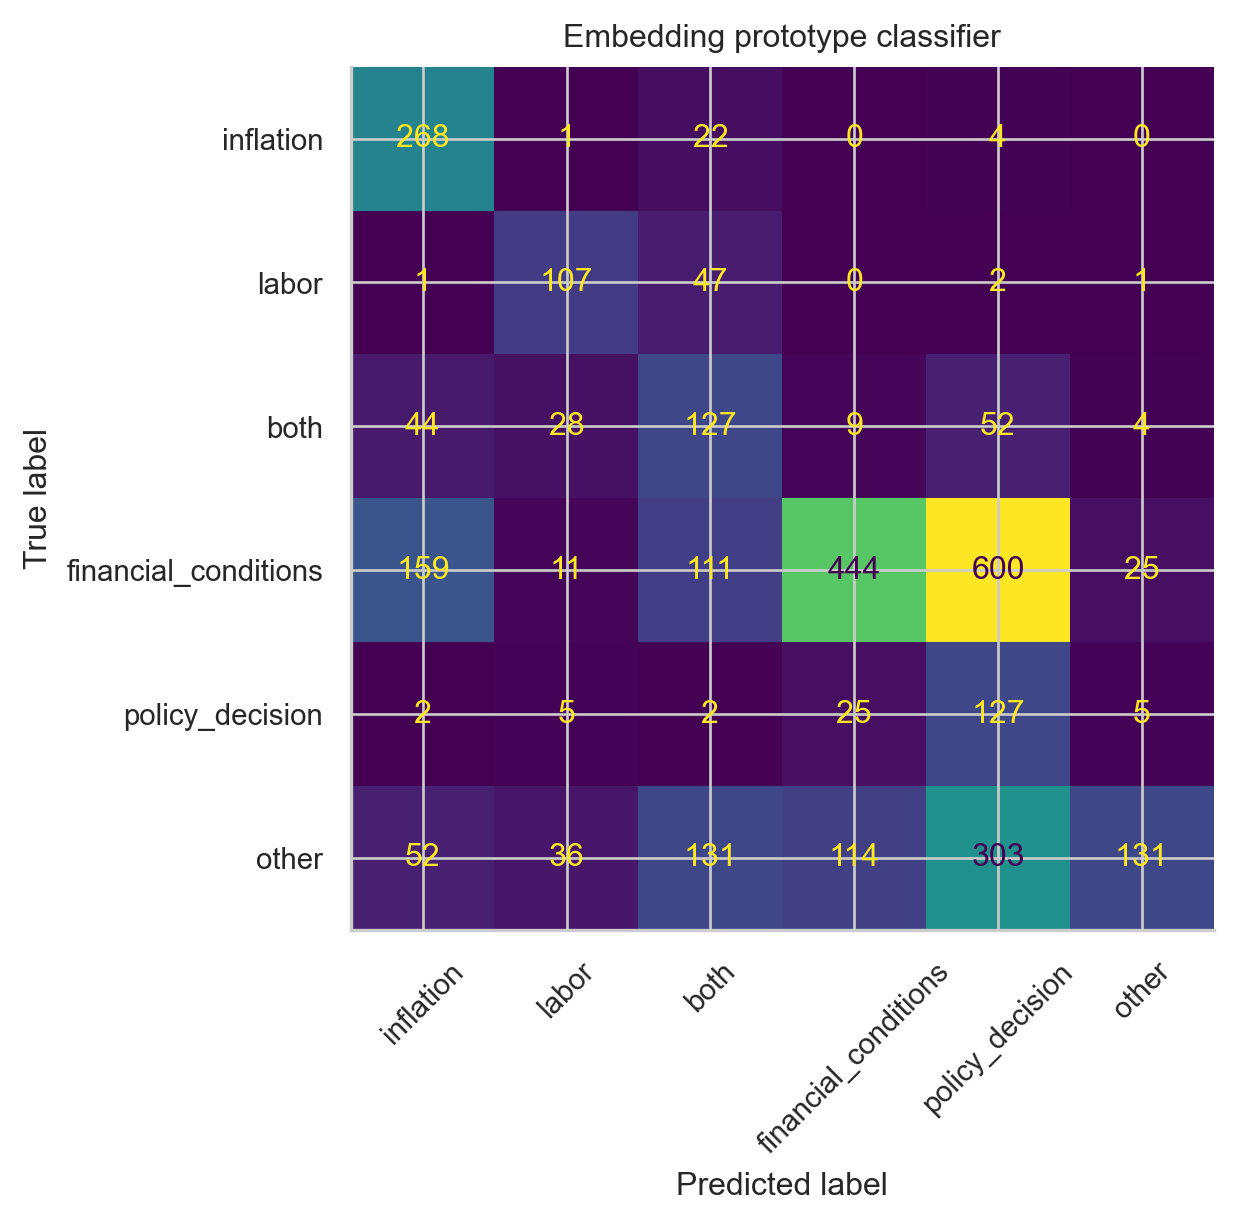
\includegraphics[width=0.7\linewidth]{figures/embedding_prototype_confusion.png}
    \caption{Embedding classifier on the pseudo-labelled sentence sample no-training baseline: each sentence is assigned to the nearest topic prototype.}
    \label{fig:placeholder}
\end{figure}
I then train small sentence classifiers on the pseudo-labels. The question is direct: can the sentence topics be learned from
text, and do embeddings add information beyond exact dictionary matching? The target is
the main topic, with \emph{other} and \emph{policy decision} merged into a single
non-mandate category when the class sizes are too small.

I compare three models. The first is the dictionary rule itself. It is transparent and
uses sentences that contain inflation or labor terms. The second is a \tfidf{}
logistic-regression classifier with unigrams and bigrams. This tests whether a standard
sparse text representation can learn the pseudo-labels. The third is a
logistic-regression classifier on local sentence embeddings from \code{nomic-embed-text}.
This tests whether semantic features capture nearby language, for example market stress
or liquidity language, outside the dictionary. I also include a no-training embedding
baseline: each sentence embedding is compared with short prototype descriptions of
inflation, labor, financial conditions, policy decisions, and other text.


\reportfigure{figures/sentence_classifier_scores.png}{0.72}
{Sentence-level classifier scores. Macro-F1 is the main metric because the pseudo-labels are unevenly distributed.}

\reportfigure{figures/sentence_classifier_confusion_embedding.png}{0.66}
{Confusion matrix for the embedding logistic-regression sentence classifier.}

\begin{table}[H]
\centering
\caption{Sentence-topic classification against LLM-assisted weak labels.}
\label{tab:sentence-classifier}
\begin{tabular}{lrr}
\toprule
Model & Accuracy & Macro-F1 \\
\midrule
Dictionary rule & 0.535 & 0.526 \\
\tfidf{} + logistic regression & 0.718 & 0.724 \\
Embedding + logistic regression & 0.768 & 0.765 \\
\bottomrule
\end{tabular}
\end{table}

The comparison gives the expected ordering. The dictionary rule is useful but limited by
exact matching. The \tfidf{} classifier improves substantially, and the embedding
classifier performs slightly better again. These numbers should not be read as accuracy
against a human-coded ground truth. They measure agreement with the LLM-assisted weak
labels. The useful result is comparative: sentence topics contain recoverable structure
beyond exact dictionary hits, and embeddings help capture some of that structure.

\subsection{Applying the classifier to the corpus}

After fitting the selected sentence classifier, I apply it to the full sentence corpus.
When full sentence embeddings are available, I use the embedding classifier. Otherwise,
the notebook falls back to the \tfidf{} classifier. In the results reported here, full
embeddings are available and the full corpus is classified with the embedding logistic
model. The resulting file \code{data/processed/fomc\_sentence\_topic\_predictions.csv}
keeps the predicted topic, prediction confidence, date, year, document type, period, and
election-window variables for each sentence.

\reportfigure{figures/embedding_topic_shares_by_document_type.png}{0.78}
{Predicted sentence-topic shares for statements and minutes. The classifier view keeps the inflation--labor contrast but adds financial conditions and policy-decision language.}

\reportfigure{figures/embedding_topic_shares_over_time.png}{0.82}
{Predicted sentence-topic shares over time. The figure focuses on inflation, labor, and financial conditions to keep the plot readable.}

\reportfigure{figures/dictionary_vs_embedding_balance.png}{0.72}
{Dictionary inflation-minus-labor balance against the classifier inflation-minus-labor sentence share. Each point is a meeting-document pair.}

This full-corpus step is the bridge between the old score and the new classifier. The
dictionary balance remains important because it has a direct interpretation. The
classifier adds a second view: whether the same meeting looks inflation-heavy or
labor-heavy after sentences are classified by broader semantic features. In the full
corpus, the classifier predicts a large financial-conditions share, especially in
minutes: 49.4\% of minutes sentences against 24.6\% of statement sentences. Statements
have more sentences that combine both sides of the mandate, 17.9\% against 5.0\% in
minutes.

The absolute levels should be read cautiously because the classifier is trained on a
small, deliberately balanced weak-label sample. The more useful comparison is relative:
the model assigns a larger financial-conditions share to minutes than to statements, and
it assigns a larger combined-mandate share to statements than to minutes. This is
consistent with the document-format interpretation: statements compress the public
message, while minutes contain more background discussion.

\subsection{Election and institutional timing}

Finally, I add a small calendar check. I mark presidential election years, midterm years,
meetings within 90 days of a federal election, the first meeting of each year, even-year
Board-cycle years, and Chair appointment or reappointment years. These variables are
descriptive calendar markers for comparing topic mix around scheduled institutional and
electoral dates.

\reportfigure{figures/election_window_dictionary_balance.png}{0.72}
{Dictionary balance inside and outside 90-day federal election windows. Points are meetings; diamonds are group means.}

\reportfigure{figures/election_window_embedding_topics.png}{0.78}
{Predicted sentence-topic shares inside and outside 90-day federal election windows.}

The reason to include this check is simple. FOMC communication is public and scheduled,
and some meetings occur close to major political events or institutional calendar points.
A visible shift in the topic mix around those dates would be worth noticing. Here the
comparison is descriptive, with a small sample and coarse timing. In this sample, the
differences are small: the predicted topic shares inside and outside 90-day election
windows are almost identical, and the dictionary balance changes little. This is not
evidence about political influence. It is a negative descriptive check around scheduled
calendar windows.

\section{Discussion}
\label{sec:discussion}

The main result is simple. Statements and minutes allocate attention differently.
Statements are short and more inflation-dominant. Minutes are longer, more diffuse, and
closer to balance. The statement--minutes gap is itself informative because it shows how
much the immediate policy message differs from the longer meeting account.

The point is not established by one number only. The dictionary score gives the most
transparent measure. The term audit shows which expressions drive the score. The
sentence audit checks whether document-level balances correspond to identifiable
sentences. The low-rank \tfidf{} map shows that document format is a major source of
variation. The weak-label sentence classifier then adds a semantic check: broader topics,
especially financial conditions, can be recovered from sentence text even when exact
inflation or labor-market terms are absent. These checks do not prove a causal story,
but they make the descriptive result more credible.

The result is also expected. Inflation is the part of the dual mandate most directly tied
to the Fed's credibility and to expectations. That makes it natural for statements to put
inflation language in the foreground, especially when the Committee is explaining the
policy decision. Labor-market language is still present, but it often works differently:
it helps describe slack, demand, wages, and the cost of tightening. The two sides of the
mandate are communicated through different textual roles.

The sentence-level results show why the dictionary should not be the whole analysis. In
some periods, especially stress periods, many important sentences are about financial
conditions, credit, market functioning, and liquidity. These sentences are relevant to
FOMC communication, but they are not inflation or labor-market sentences in the narrow
dictionary sense. The balance score is therefore best read as a descriptive measure of
inflation-versus-labor attention, while the sentence classifier adds a third dimension
that explains part of what the dictionary leaves out.

The rate-decision and period figures move in plausible directions. Hike meetings are
more inflation-heavy than cut meetings, and the Covid shock is one of the clearest points
where labor-market language becomes more visible. These are associations in a small
sample, not causal estimates. The election-window check is similar. It is included as a
calendar comparison, and the result is mostly negative: in this sample, the topic mix
inside and outside 90-day federal election windows looks very similar.

The main methodological lesson is that document format matters. Models that pool
statements and minutes can mainly learn the difference between a short public statement
and a long meeting summary. This is why the report keeps the dictionary score separated
by document type and uses sentence models as a check rather than as a replacement. The
methods point in the same general direction, but each has a different weakness. The
conclusion should therefore be read as a triangulated descriptive finding, not as a
single definitive measurement.

\section{Connection with the Companion Report}
\label{sec:companion}

This report and the companion hawkish/dovish report share the same corpus, but they
measure different objects. The mandate balance asks what macro topic is emphasized:
inflation or the labor market. The hawkish/dovish score asks what policy signal the text
sends. Keeping the two dimensions separate avoids treating all inflation language as
hawkish and all labor-market language as dovish.

\section{Conclusion}
\label{sec:conclusion}

In this sample of 199 \fomc{} meetings, statements and minutes give different textual
weights to the two sides of the dual mandate. Statements are much shorter and more
inflation-dominant. Minutes are more balanced and contain a wider discussion. This is the
main descriptive result of the report.

Several checks point in the same direction. The dictionary balance is higher in
statements. The term audit shows that the result is driven by economically meaningful
expressions, even though the word \emph{inflation} plays a large role. The
sentence-level dictionary audit shows that statements more often compress inflation and
labor-market language into the same short document. The low-rank \tfidf{} map shows that
statements and minutes are different textual formats. The weak-label sentence classifier
adds one more check: broader sentence topics are partly learnable from text, and
embedding features agree more closely with the weak labels than the dictionary rule.

The qualification is important. The inflation--labor contrast does not cover all of
FOMC communication. In stress periods, financial conditions become central, and a pure
dual-mandate dictionary misses that part of the story. The classifier view helps make
this visible, especially in minutes. Its absolute topic shares should be read cautiously
because the model is trained on a small weakly labelled sample, but the comparison with
the dictionary is useful.

The report therefore supports a cautious conclusion. Public FOMC communication in this
sample puts more relative inflation emphasis in statements than in minutes. Minutes give
a broader account of the meeting, including more labor-market and financial-conditions
language. This does not identify the Fed's objective function, and it does not make a
causal claim about policy or politics. It is a descriptive NLP result: different public
documents from the same meetings allocate textual attention differently, and simple
machine-learning tools help check where the transparent dictionary measure is reliable
and where it is incomplete.

\appendix

\section{\tfidf{} Sanity Check}
\label{app:tfidf}

\reportfigure{figures/model_macro_f1.png}{0.90}
{Macro-F1 scores for \tfidf{} models. The dashed line is the majority-class baseline.}

A small \tfidf{} classification exercise remains in the appendix. The target is either
the current rate decision or the next meeting's rate decision. The models are standard
\tfidf{}+\logreg{} and \tfidf{}+\svm{} classifiers, compared with a majority-class
baseline. The split is chronological: the first 70\% of meetings are used for training
and the last 30\% for testing.

The rate-decision scores remain modest. The majority baseline has macro-F1 0.222. For
the current decision, the best model is \tfidf{}+\svm{} on full minutes, with macro-F1
0.418. For the next decision, the best model is again based on minutes, with macro-F1
0.396.

This exercise is a small appendix check. The sample has 199 meetings, the classes are
unbalanced, and minutes are released after the meeting. The main takeaway is smaller:
minutes contain more decision-related context than statements, even though statements
have a higher density of mandate terms.

\section{Document-Level Embedding Check}
\label{app:embeddings}

\reportfigure{figures/embedding_dictionary_balance.png}{0.72}
{Dictionary balance against embedding prototype balance.}

\reportfigure{figures/embedding_pca_map.png}{0.72}
{PCA map of local document embeddings. Color is the embedding prototype balance.}

Before the sentence-level model, I also tried a small local embedding check with
\code{nomic-embed-text}. Each document is represented by a short beginning/middle/end
excerpt, and the document vector is compared with one inflation prototype phrase and one
labor-market prototype phrase. This document-level view is noisier than the sentence
classifier, especially for minutes, so I keep it in the appendix. It points to the same
message as the LSA map: statements and minutes are different document formats. The main
embedding result in the report is now the sentence-level classifier in
\cref{sec:sentence-classifier}.

\newpage

\begin{thebibliography}{99}

\bibitem[Acosta and Meade(2015)]{acosta2015hanging}
Acosta, M., and Meade, E. E.
\newblock Hanging on every word: Semantic analysis of the FOMC's postmeeting statement.
\newblock \emph{FEDS Notes}, Board of Governors of the Federal Reserve System, 2015.

\bibitem[Blinder et~al.(2008)]{blinder2008central}
Blinder, A. S., Ehrmann, M., Fratzscher, M., De Haan, J., and Jansen, D.-J.
\newblock Central bank communication and monetary policy: A survey of theory and evidence.
\newblock \emph{Journal of Economic Literature}, 46(4):910--945, 2008.

\bibitem[Deerwester et~al.(1990)]{deerwester1990indexing}
Deerwester, S., Dumais, S. T., Furnas, G. W., Landauer, T. K., and Harshman, R.
\newblock Indexing by latent semantic analysis.
\newblock \emph{Journal of the American Society for Information Science}, 41(6):391--407, 1990.

\bibitem[Doh et~al.(2021)]{doh2021matters}
Doh, T., Kim, S., and Yang, S.-K.
\newblock How you say it matters: Text analysis of FOMC statements using natural language processing.
\newblock \emph{Economic Review, Federal Reserve Bank of Kansas City}, 106(1):25--40, 2021.

\bibitem[Doh et~al.(forthcoming)]{doh2025deciphering}
Doh, T., Song, D., and Yang, S.-K.
\newblock Deciphering Federal Reserve communication via text analysis of alternative FOMC statements.
\newblock \emph{American Economic Journal: Macroeconomics}, forthcoming.

\bibitem[Gentzkow et~al.(2019)]{gentzkow2019text}
Gentzkow, M., Kelly, B., and Taddy, M.
\newblock Text as data.
\newblock \emph{Journal of Economic Literature}, 57(3):535--574, 2019.

\bibitem[Hansen et~al.(2018)]{hansen2018transparency}
Hansen, S., McMahon, M., and Prat, A.
\newblock Transparency and deliberation within the FOMC: A computational linguistics approach.
\newblock \emph{The Quarterly Journal of Economics}, 133(2):801--870, 2018.

\bibitem[Loughran and McDonald(2011)]{loughran2011liability}
Loughran, T., and McDonald, B.
\newblock When is a liability not a liability? Textual analysis, dictionaries, and 10-Ks.
\newblock \emph{Journal of Finance}, 66(1):35--65, 2011.

\bibitem[Shapiro and Wilson(2022)]{shapiro2022taking}
Shapiro, A. H., and Wilson, D. J.
\newblock Taking the Fed at its word: A new approach to estimating central bank objectives using text analysis.
\newblock \emph{The Review of Economic Studies}, 89(5):2768--2805, 2022.

\bibitem[Tadle(2022)]{tadle2022minutes}
Tadle, R. C.
\newblock FOMC minutes sentiments and their impact on financial markets.
\newblock \emph{Journal of Economics and Business}, 118:106021, 2022.

\end{thebibliography}

\end{document}
